\documentclass[tikz,border=18pt]{standalone}
\usepackage{fontspec}
\setmainfont{Arial}
\usetikzlibrary{arrows.meta,positioning,calc}

\definecolor{navy}{RGB}{15,23,42}
\definecolor{slate}{RGB}{71,85,105}
\definecolor{line}{RGB}{203,213,225}
\definecolor{danger}{RGB}{220,38,38}
\definecolor{dangerbg}{RGB}{254,242,242}
\definecolor{blue}{RGB}{2,132,199}
\definecolor{bluebg}{RGB}{240,249,255}
\definecolor{green}{RGB}{5,150,105}
\definecolor{greenbg}{RGB}{236,253,245}

\begin{document}
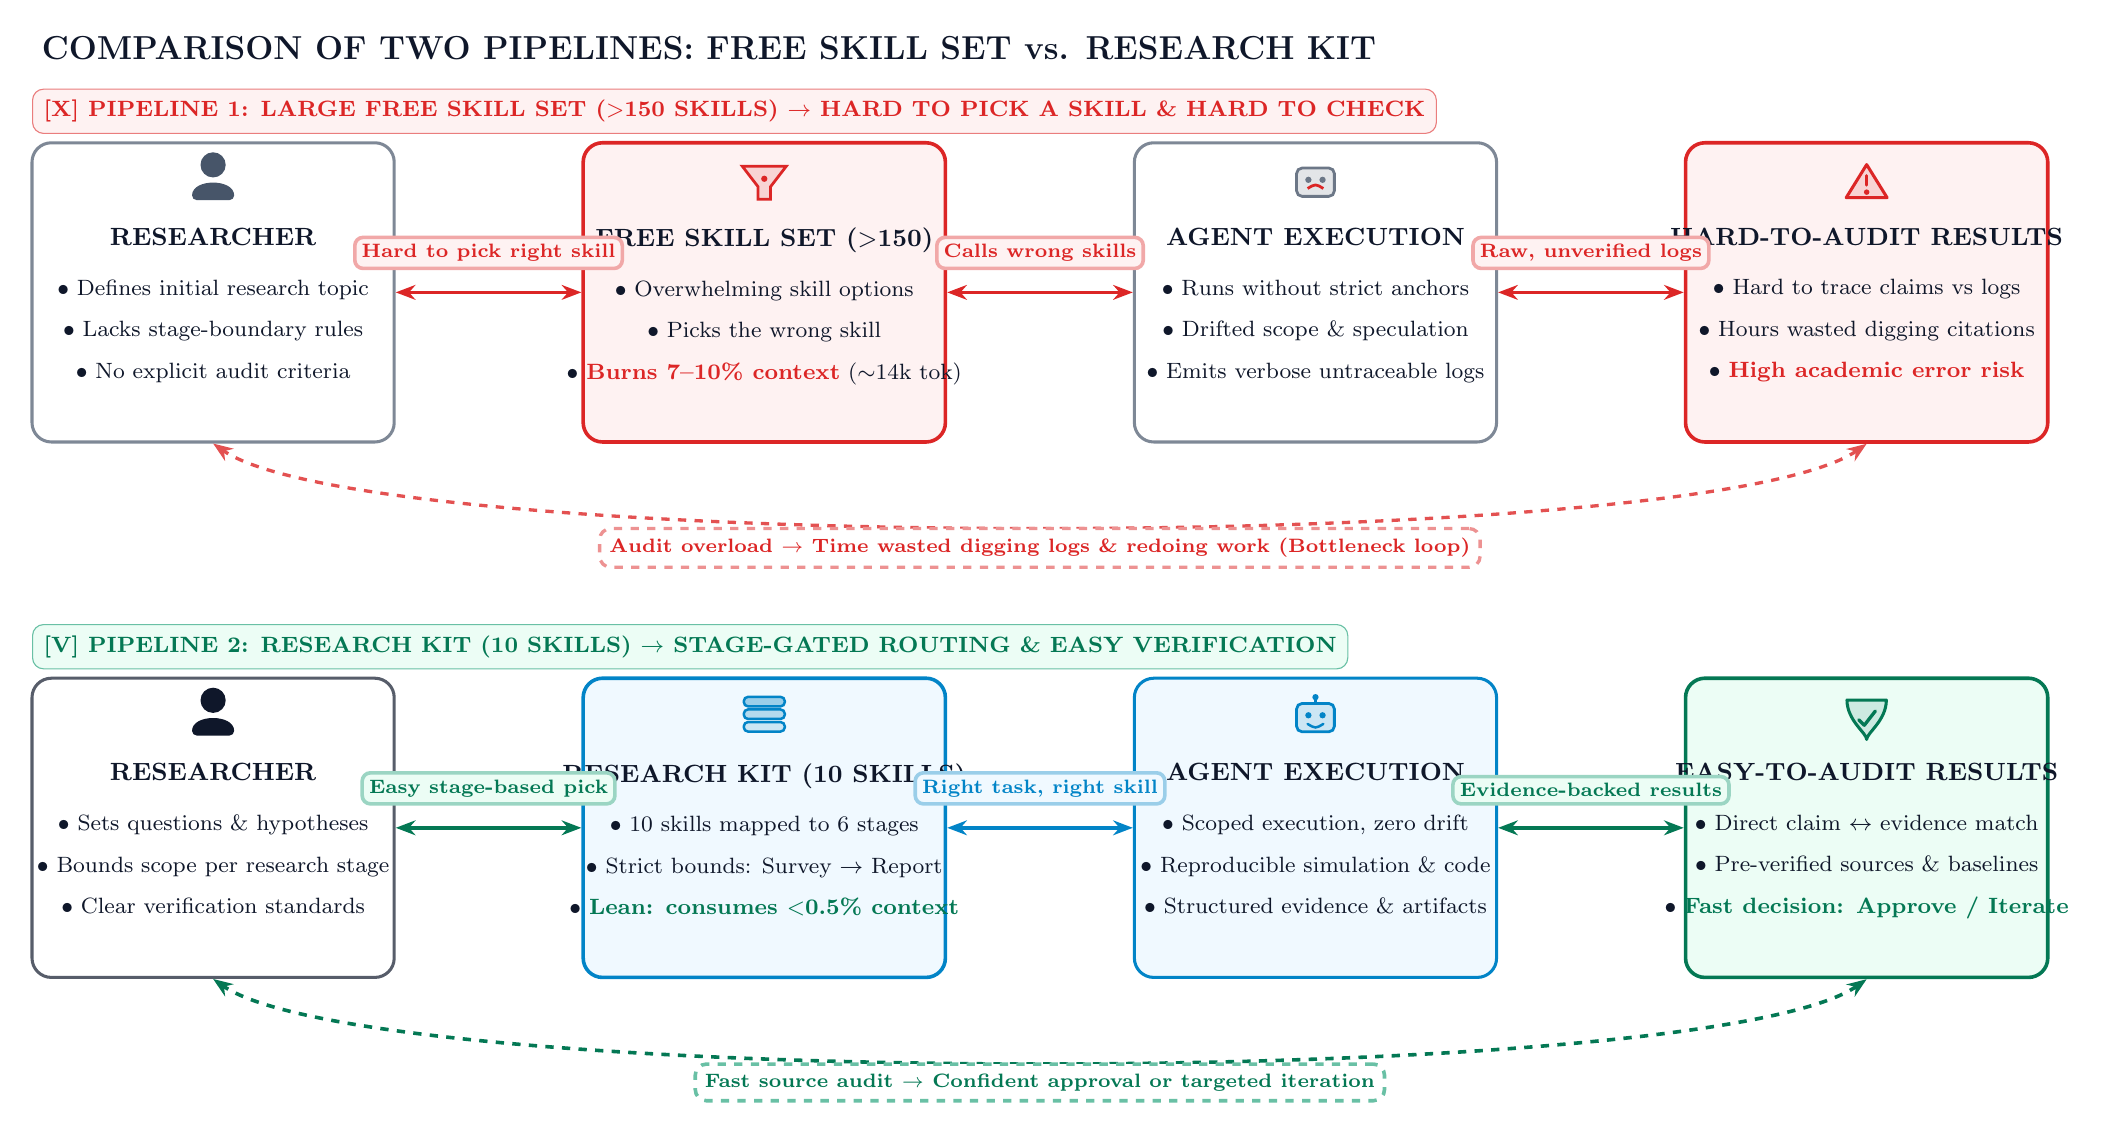
\begin{tikzpicture}[
  >=Stealth,
  % Row 1 styles (Bloated / Problematic)
  card1/.style={draw=slate!70, fill=white, rounded corners=7pt, line width=1.1pt,
    minimum width=4.6cm, minimum height=3.8cm, align=center, text=navy},
  skillcard1/.style={draw=danger, fill=dangerbg, rounded corners=7pt, line width=1.3pt,
    minimum width=4.6cm, minimum height=3.8cm, align=center, text=navy},
  agentcard1/.style={draw=slate!70, fill=white, rounded corners=7pt, line width=1.1pt,
    minimum width=4.6cm, minimum height=3.8cm, align=center, text=navy},
  reviewcard1/.style={draw=danger, fill=dangerbg, rounded corners=7pt, line width=1.3pt,
    minimum width=4.6cm, minimum height=3.8cm, align=center, text=navy},
  % Row 2 styles (Research Kit / Standardized)
  card2/.style={draw=navy!70, fill=white, rounded corners=7pt, line width=1.1pt,
    minimum width=4.6cm, minimum height=3.8cm, align=center, text=navy},
  skillcard2/.style={draw=blue, fill=bluebg, rounded corners=7pt, line width=1.3pt,
    minimum width=4.6cm, minimum height=3.8cm, align=center, text=navy},
  agentcard2/.style={draw=blue, fill=bluebg, rounded corners=7pt, line width=1.1pt,
    minimum width=4.6cm, minimum height=3.8cm, align=center, text=navy},
  reviewcard2/.style={draw=green!80!black, fill=greenbg, rounded corners=7pt, line width=1.3pt,
    minimum width=4.6cm, minimum height=3.8cm, align=center, text=navy}
]

  % Top Main Title
  \node[anchor=west, font=\large\bfseries, text=navy] at (-12.8, 6.7)
    {COMPARISON OF TWO PIPELINES: FREE SKILL SET vs. RESEARCH KIT};

  % =========================================================================
  % ROW 1: BLOATED OPEN CATALOG (>150 SKILLS) - BOTTLENECK & HARD TO REVIEW
  % =========================================================================
  \node[anchor=west, font=\footnotesize\bfseries, fill=dangerbg, draw=danger!60, rounded corners=4pt, inner sep=4pt, text=danger] at (-12.8, 5.9)
    {[X] PIPELINE 1: LARGE FREE SKILL SET ($>$150 SKILLS) $\rightarrow$ HARD TO PICK A SKILL \& HARD TO CHECK};

  % 1.1 Researcher 1
  \node[card1] (human1) at (-10.5, 3.6) {};
  \begin{scope}[shift={($(human1.north)+(0, -0.52)$)}]
    \fill[slate] (0, 0.22) circle (0.16cm);
    \draw[fill=slate, draw=slate, rounded corners=1.5pt] (-0.26, -0.22) .. controls (-0.26, 0.04) and (0.26, 0.04) .. (0.26, -0.22) -- cycle;
  \end{scope}
  \node[anchor=north, align=center, text=navy] at ($(human1.north)+(0, -0.98)$) {
    \textbf{\small RESEARCHER}\\[6pt]
    \footnotesize $\bullet$ Defines initial research topic\\[3pt]
    \footnotesize $\bullet$ Lacks stage-boundary rules\\[3pt]
    \footnotesize $\bullet$ No explicit audit criteria
  };

  % 1.2 Skill 1
  \node[skillcard1] (skill1) at (-3.5, 3.6) {};
  \begin{scope}[shift={($(skill1.north)+(0, -0.52)$)}]
    \draw[draw=danger, fill=danger!20, line width=1pt] (-0.28, 0.20) -- (0.28, 0.20) -- (0.08, -0.06) -- (0.08, -0.22) -- (-0.08, -0.22) -- (-0.08, -0.06) -- cycle;
    \fill[danger] (0, 0.04) circle (0.04cm);
  \end{scope}
  \node[anchor=north, align=center, text=navy] at ($(skill1.north)+(0, -0.98)$) {
    \textbf{\small FREE SKILL SET ($>$150)}\\[6pt]
    \footnotesize $\bullet$ Overwhelming skill options\\[3pt]
    \footnotesize $\bullet$ Picks the wrong skill\\[3pt]
    \footnotesize $\bullet$ \textcolor{danger}{\textbf{Burns 7--10\% context}} ($\sim$14k tok)
  };

  % 1.3 Agent 1
  \node[agentcard1] (agent1) at (3.5, 3.6) {};
  \begin{scope}[shift={($(agent1.north)+(0, -0.52)$)}]
    \draw[draw=slate!80, fill=slate!15, rounded corners=2pt, line width=1pt] (-0.24, -0.18) rectangle (0.24, 0.18);
    \fill[slate!80] (-0.09, 0.03) circle (0.04cm);
    \fill[slate!80] (0.09, 0.03) circle (0.04cm);
    \draw[draw=danger, line width=1pt] (-0.10, -0.08) .. controls (0, -0.02) .. (0.10, -0.08);
  \end{scope}
  \node[anchor=north, align=center, text=navy] at ($(agent1.north)+(0, -0.98)$) {
    \textbf{\small AGENT EXECUTION}\\[6pt]
    \footnotesize $\bullet$ Runs without strict anchors\\[3pt]
    \footnotesize $\bullet$ Drifted scope \& speculation\\[3pt]
    \footnotesize $\bullet$ Emits verbose untraceable logs
  };

  % 1.4 Review 1
  \node[reviewcard1] (review1) at (10.5, 3.6) {};
  \begin{scope}[shift={($(review1.north)+(0, -0.52)$)}]
    \draw[draw=danger, fill=danger!20, line width=1.1pt, line join=round] (0, 0.22) -- (0.26, -0.20) -- (-0.26, -0.20) -- cycle;
    \draw[draw=danger, line width=1.1pt, line cap=round] (0, 0.08) -- (0, -0.04);
    \fill[danger] (0, -0.13) circle (0.035cm);
  \end{scope}
  \node[anchor=north, align=center, text=navy] at ($(review1.north)+(0, -0.98)$) {
    \textbf{\small HARD-TO-AUDIT RESULTS}\\[6pt]
    \footnotesize $\bullet$ Hard to trace claims vs logs\\[3pt]
    \footnotesize $\bullet$ Hours wasted digging citations\\[3pt]
    \footnotesize $\bullet$ \textcolor{danger}{\textbf{High academic error risk}}
  };

  % Row 1 Arrows
  \draw[{Stealth[length=2.5mm]}-{Stealth[length=2.5mm]}, line width=1.3pt, draw=danger] 
    (human1.east) -- (skill1.west)
    node[midway, above=8pt, fill=dangerbg, draw=danger!40, rounded corners=3pt, inner sep=2.5pt, font=\scriptsize\bfseries, text=danger] {Hard to pick right skill};

  \draw[{Stealth[length=2.5mm]}-{Stealth[length=2.5mm]}, line width=1.3pt, draw=danger] 
    (skill1.east) -- (agent1.west)
    node[midway, above=8pt, fill=dangerbg, draw=danger!40, rounded corners=3pt, inner sep=2.5pt, font=\scriptsize\bfseries, text=danger] {Calls wrong skills};

  \draw[{Stealth[length=2.5mm]}-{Stealth[length=2.5mm]}, line width=1.3pt, draw=danger] 
    (agent1.east) -- (review1.west)
    node[midway, above=8pt, fill=dangerbg, draw=danger!40, rounded corners=3pt, inner sep=2.5pt, font=\scriptsize\bfseries, text=danger] {Raw, unverified logs};

  % Row 1 Feedback Loop
  \draw[{Stealth[length=2.5mm]}-{Stealth[length=2.5mm]}, line width=1.2pt, draw=danger!80, dashed] (review1.south) to[out=-145, in=-35, looseness=0.30] 
    node[midway, below, font=\scriptsize\bfseries, text=danger, fill=white, inner sep=3.5pt, rounded corners=4pt, draw=danger!50] 
    {Audit overload $\rightarrow$ Time wasted digging logs \& redoing work (Bottleneck loop)}
    (human1.south);


  % =========================================================================
  % ROW 2: RESEARCH KIT (10 SKILLS) - LEAN, STAGE-BASED & EASY TO AUDIT
  % =========================================================================
  \node[anchor=west, font=\footnotesize\bfseries, fill=greenbg, draw=green!60, rounded corners=4pt, inner sep=4pt, text=green!80!black] at (-12.8, -0.9)
    {[V] PIPELINE 2: RESEARCH KIT (10 SKILLS) $\rightarrow$ STAGE-GATED ROUTING \& EASY VERIFICATION};

  % 2.1 Researcher 2
  \node[card2] (human2) at (-10.5, -3.2) {};
  \begin{scope}[shift={($(human2.north)+(0, -0.52)$)}]
    \fill[navy] (0, 0.22) circle (0.16cm);
    \draw[fill=navy, draw=navy, rounded corners=1.5pt] (-0.26, -0.22) .. controls (-0.26, 0.04) and (0.26, 0.04) .. (0.26, -0.22) -- cycle;
  \end{scope}
  \node[anchor=north, align=center, text=navy] at ($(human2.north)+(0, -0.98)$) {
    \textbf{\small RESEARCHER}\\[6pt]
    \footnotesize $\bullet$ Sets questions \& hypotheses\\[3pt]
    \footnotesize $\bullet$ Bounds scope per research stage\\[3pt]
    \footnotesize $\bullet$ Clear verification standards
  };

  % 2.2 Skill 2
  \node[skillcard2] (skill2) at (-3.5, -3.2) {};
  \begin{scope}[shift={($(skill2.north)+(0, -0.52)$)}]
    \draw[draw=blue, fill=blue!20, rounded corners=1.5pt, line width=0.9pt] (-0.26, -0.18) rectangle (0.26, -0.06);
    \draw[draw=blue, fill=blue!30, rounded corners=1.5pt, line width=0.9pt] (-0.26, -0.02) rectangle (0.26, 0.10);
    \draw[draw=blue, fill=blue!40, rounded corners=1.5pt, line width=0.9pt] (-0.26, 0.14) rectangle (0.26, 0.26);
  \end{scope}
  \node[anchor=north, align=center, text=navy] at ($(skill2.north)+(0, -0.98)$) {
    \textbf{\small RESEARCH KIT (10 SKILLS)}\\[6pt]
    \footnotesize $\bullet$ 10 skills mapped to 6 stages\\[3pt]
    \footnotesize $\bullet$ Strict bounds: Survey $\rightarrow$ Report\\[3pt]
    \footnotesize $\bullet$ \textcolor{green!80!black}{\textbf{Lean: consumes $<$0.5\% context}}
  };

  % 2.3 Agent 2
  \node[agentcard2] (agent2) at (3.5, -3.2) {};
  \begin{scope}[shift={($(agent2.north)+(0, -0.52)$)}]
    \draw[draw=blue, fill=blue!20, rounded corners=2pt, line width=1pt] (-0.24, -0.18) rectangle (0.24, 0.18);
    \draw[draw=blue, line width=0.9pt] (0, 0.18) -- (0, 0.26);
    \fill[blue] (0, 0.26) circle (0.04cm);
    \fill[blue] (-0.09, 0.03) circle (0.04cm);
    \fill[blue] (0.09, 0.03) circle (0.04cm);
    \draw[draw=blue, line width=0.9pt, line cap=round] (-0.10, -0.08) .. controls (0, -0.14) .. (0.10, -0.08);
  \end{scope}
  \node[anchor=north, align=center, text=navy] at ($(agent2.north)+(0, -0.98)$) {
    \textbf{\small AGENT EXECUTION}\\[6pt]
    \footnotesize $\bullet$ Scoped execution, zero drift\\[3pt]
    \footnotesize $\bullet$ Reproducible simulation \& code\\[3pt]
    \footnotesize $\bullet$ Structured evidence \& artifacts
  };

  % 2.4 Review 2
  \node[reviewcard2] (review2) at (10.5, -3.2) {};
  \begin{scope}[shift={($(review2.north)+(0, -0.52)$)}]
    \draw[draw=green!80!black, fill=green!20, line width=1.1pt, line join=round] 
      (-0.25, 0.22) -- (0.25, 0.22) .. controls (0.25, -0.04) and (0, -0.20) .. (0, -0.28) .. controls (0, -0.20) and (-0.25, -0.04) .. (-0.25, 0.22) -- cycle;
    \draw[draw=green!80!black, line width=1.2pt, line cap=round, line join=round] 
      (-0.10, -0.03) -- (-0.03, -0.10) -- (0.11, 0.08);
  \end{scope}
  \node[anchor=north, align=center, text=navy] at ($(review2.north)+(0, -0.98)$) {
    \textbf{\small EASY-TO-AUDIT RESULTS}\\[6pt]
    \footnotesize $\bullet$ Direct claim $\leftrightarrow$ evidence match\\[3pt]
    \footnotesize $\bullet$ Pre-verified sources \& baselines\\[3pt]
    \footnotesize $\bullet$ \textcolor{green!80!black}{\textbf{Fast decision: Approve / Iterate}}
  };

  % Row 2 Arrows
  \draw[{Stealth[length=2.5mm]}-{Stealth[length=2.5mm]}, line width=1.3pt, draw=green!80!black] 
    (human2.east) -- (skill2.west)
    node[midway, above=8pt, fill=greenbg, draw=green!40, rounded corners=3pt, inner sep=2.5pt, font=\scriptsize\bfseries, text=green!80!black] {Easy stage-based pick};

  \draw[{Stealth[length=2.5mm]}-{Stealth[length=2.5mm]}, line width=1.3pt, draw=blue] 
    (skill2.east) -- (agent2.west)
    node[midway, above=8pt, fill=bluebg, draw=blue!40, rounded corners=3pt, inner sep=2.5pt, font=\scriptsize\bfseries, text=blue] {Right task, right skill};

  \draw[{Stealth[length=2.5mm]}-{Stealth[length=2.5mm]}, line width=1.3pt, draw=green!80!black] 
    (agent2.east) -- (review2.west)
    node[midway, above=8pt, fill=greenbg, draw=green!40, rounded corners=3pt, inner sep=2.5pt, font=\scriptsize\bfseries, text=green!80!black] {Evidence-backed results};

  % Row 2 Feedback Loop
  \draw[{Stealth[length=2.5mm]}-{Stealth[length=2.5mm]}, line width=1.3pt, draw=green!80!black, dashed] (review2.south) to[out=-145, in=-35, looseness=0.30] 
    node[midway, below, font=\scriptsize\bfseries, text=green!80!black, fill=white, inner sep=3.5pt, rounded corners=4pt, draw=green!60] 
    {Fast source audit $\rightarrow$ Confident approval or targeted iteration}
    (human2.south);

\end{tikzpicture}
\end{document}
